\documentclass[tikz,border=8pt]{standalone}
% Shared look for every TikZ diagram. Load with \input{../../tools/tikz-style.tex}
\usepackage[T1]{fontenc}
\usepackage{lmodern}
\renewcommand{\sfdefault}{lmr}  % diagrams use the same serif as the text
\usetikzlibrary{arrows.meta, positioning, shapes.geometric, calc, fit, backgrounds}
\definecolor{cblue}{HTML}{4C78A8}
\definecolor{corange}{HTML}{F58518}
\definecolor{cgreen}{HTML}{54A24B}
\definecolor{cred}{HTML}{E45756}
\definecolor{cpurple}{HTML}{B279A2}
\definecolor{cgrey}{HTML}{6B6B6B}
\tikzset{
  every picture/.style={font=\sffamily, line width=1.2pt},
  box/.style={draw=#1, fill=#1!12, rounded corners=4pt, align=center, inner sep=7pt, minimum height=1.1cm},
  box/.default=cgrey,
  arrow/.style={-{Stealth[length=3mm]}, draw=cgrey, line width=1.4pt},
  title/.style={font=\sffamily\bfseries\Large},
  note/.style={font=\sffamily\small, text=cgrey, align=center},
}
\AtBeginDocument{\hyphenpenalty=10000 \exhyphenpenalty=10000}

\begin{document}
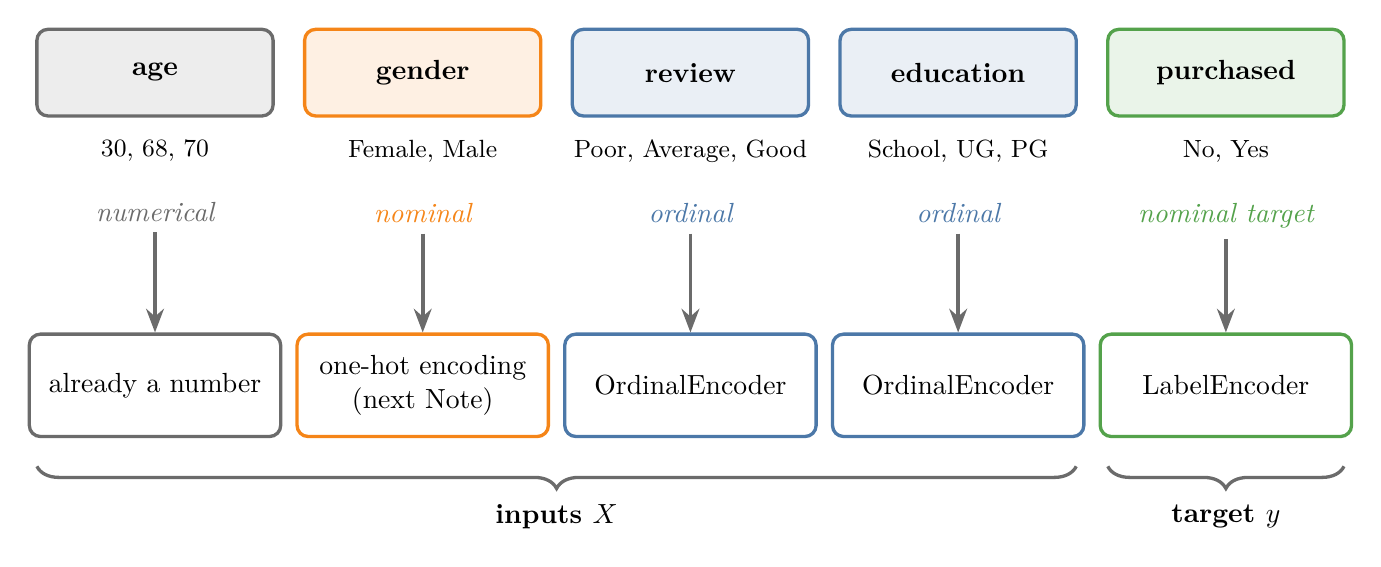
\begin{tikzpicture}
  \foreach \x/\h/\c/\t/\e/\v in {
      0/age/cgrey/numerical/already a number/{30, 68, 70},
      3.4/gender/corange/nominal/one-hot encoding\\(next Note)/{Female, Male},
      6.8/review/cblue/ordinal/OrdinalEncoder/{Poor, Average, Good},
      10.2/education/cblue/ordinal/OrdinalEncoder/{School, UG, PG},
      13.6/purchased/cgreen/nominal target/LabelEncoder/{No, Yes}} {
    \node[box=\c, font=\sffamily\bfseries, minimum width=3.0cm] (h) at (\x,0) {\h};
    \node[note, text=black, text width=3.0cm, below=0.15cm of h] (v) {\v};
    \node[font=\sffamily\itshape, text=\c, below=0.25cm of v] (t) {\t};
    \node[box=\c, fill=white, text width=2.7cm, minimum height=1.3cm, anchor=north] (e) at (\x,-3.3) {\e};
    \draw[arrow] (t.south) -- (e.north);
  }
  \draw[decorate, decoration={brace, amplitude=8pt, mirror}, draw=cgrey]
    (-1.5,-5.0) -- (11.7,-5.0) node[midway, below=10pt, font=\sffamily\bfseries] {inputs $X$};
  \draw[decorate, decoration={brace, amplitude=8pt, mirror}, draw=cgrey]
    (12.1,-5.0) -- (15.1,-5.0) node[midway, below=10pt, font=\sffamily\bfseries] {target $y$};
\end{tikzpicture}
\end{document}
